% !TeX root =  main.tex

\section{Functions}

\subsection{Basic Concepts}
\begin{definition}
  A \textbf{relation} is a set of ordered pairs. The set of the first components of each ordered pair is called the \textbf{domain} and the set of the second components of each ordered pair is called the \textbf{range}.

  A \textbf{function} is a relation that assigns each element in the domain a unique element in the range.

  An arbitrary value in the domain is often represented by the lowercase letter $x$ which is called an \textbf{independent variable}.
  An arbitrary output is often represented by the lowercase letter $y$ which is called a \textbf{dependent variable}.
  
  % Each value in the domain is also known as an input value. Each value in the range is also known as an output value.
\end{definition}

\begin{example}
  Determine if the relation 
  \[\{(1,2),(2,4),(3,6),(4,8),(5,10)\}\]
  is a function. Find the domain and the range.
\end{example}

If a function has $x$ as the independent variable and $y$ as the dependent variable, then we often say that $y$ is a function of $x$.

\begin{example}
  Consider items and prices in a grocery store. Is price a function of item? Is item a function of price? 
\end{example}

  A function is often named by letters, such as $f$, $F$, $p$, or $q$. If $f$ is a function of $x$, then we denote it as $y=f(x)$ which is called the function notation. Here $f(x)$ is read as $f$ of $x$ or $f$ at $x$. The notation $f(x)$ represents the output of the function $f$ for a given input $x$.
  
\begin{example}
  Use function notation to represent a function whose input is the name of a month and output is the number of days in that month.
\end{example}

\begin{example}
  A function \(N=f(y)\) gives the number of police officers, \(N\), in a town in year \(y\). What does \(f(2005)=300\) represent?
\end{example}

\begin{example}
  Using a table to represent the days in the month as the function of month.
\end{example}

\begin{example}
  Consider the function $f(x)=x^2+3x-4$. Find the values of the following expressions.

\begin{enumerate}[fourcol]
  \item \(f(2)\)
  \item \(f(a)\)
  \item \(f(a+h)\)
  \item \(\dfrac{f(a+h)-f(a)}{h}\)
\end{enumerate}
\end{example}

\begin{example}
  Consider the function $f(x)=x^2-2x$. Find all $x$ values such that $f(x)=3$.
\end{example}

\begin{example}
  Express the relationship defined by the function $2x-y-3=0$ as a function $y=l(x)$.
\end{example}

\begin{example}
  Does the equation \(x^2+y^2=1\) defines $y$ as a function $x$. If so, express the relationship as a function \(y=f(x)\). If not, under what extra condition does the function $y=f(x)$ exist? 
\end{example}

\begin{example}
  Consider the function $f(x)$ defined by a graph below.

  \begin{multicols}{2}
    \begin{enumerate}
      \item Find $f(-1)$. 
      \item Find all $x$ such that $f(x)=3$.
    \end{enumerate}
    \vfill

    \columnbreak
    
    \begin{center}
      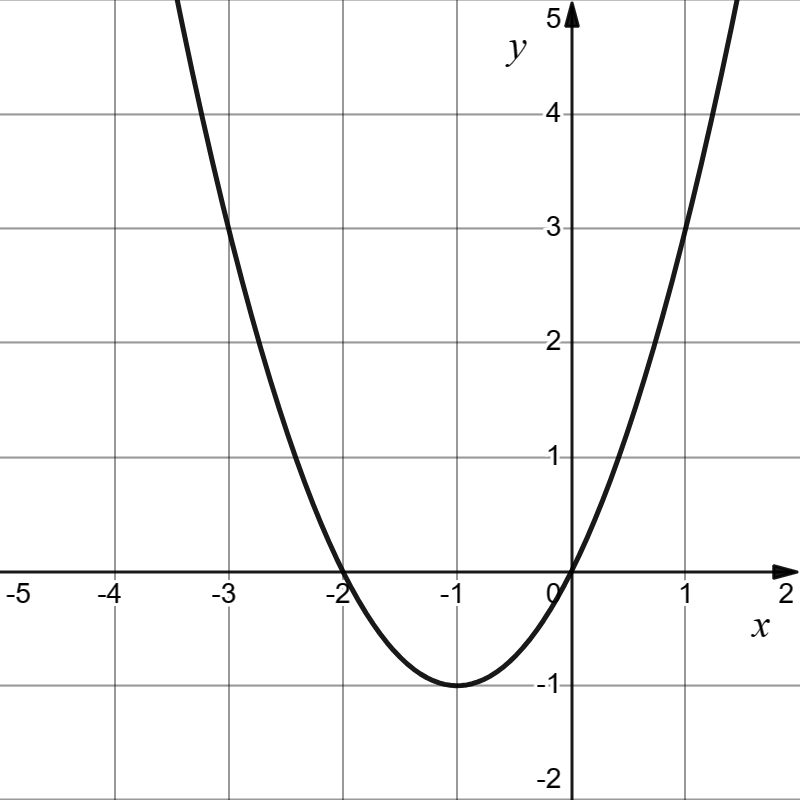
\includegraphics[scale=0.25]{figs/f(x)=x^2+2x.png}
    \end{center}
  \end{multicols}
\end{example}

\begin{definition}
  A function is a \textbf{one-to-one function} if each output value corresponds to exactly one input value.
\end{definition}

\begin{example}
  Is the area of a circle a function of its radius? If yes, is the function one-to-one?
\end{example}

A graph is a function if very vertical line crosses the graph at most once. This method is known as the \textbf{vertical line test}.

A function is an one-to-one if very horizontal line crosses the graph at most once. This method is known as the \textbf{horizontal line test}.

\begin{example}
  Determine if the graph defines a function. If so, is it a one-to-one function?
  \begin{center}
  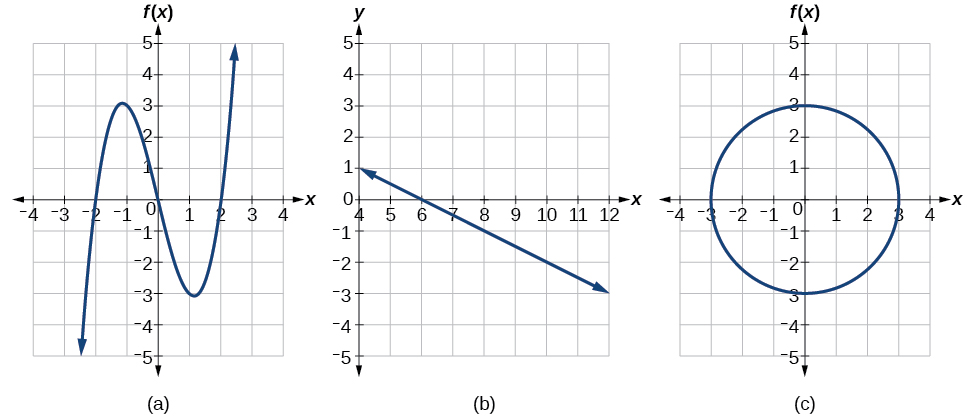
\includegraphics[width=0.8\textwidth]{figs/cubic-line-circle.jpg}
  \end{center}
\end{example}

\newpage
\section*{Exercises}

\begin{exercise}
  Consider the function $f(x)=2x^2+x-3$. Find the values of the following expressions.

\begin{enumerate}[fourcol]
  \item \(f(-1)\)
  \item \(f(a)\)
  \item \(f(a+h)\)
  \item \(\dfrac{f(a+h)-f(a)}{h}\)
\end{enumerate}
\end{exercise}
\vspace*{2\baselineskip}

\begin{exercise}
  For the function $f(x)=-4x+5$, evaluate and simplify the difference quotient $\dfrac{f(x+h)-f(x)}{h}$.
\end{exercise}
\vspace*{2\baselineskip}

\begin{exercise}
  Consider the function $f(x)=-x^2-4x$. Find all $x$ values such that $f(x)=3$.
\end{exercise}

\begin{exercise}
  Express the relationship defined by the function $3x-2y-6=0$ as a function $y=l(x)$.
\end{exercise}

\begin{exercise}
  If \(8x-y^3=0\), express \(y\) as a function of \(x\).

  Is $y$ a one-to-one function of $x$?
\end{exercise}


\begin{exercise}
  Consider the function $f(x)$ defined by a graph below.

  \begin{multicols}{2}
    \begin{enumerate}
      \item Find $f(1)$. 
      \item Find all $x$ such that $f(x)=3$.
    \end{enumerate}
    \vfill\mbox{}

    \columnbreak
    
    \begin{center}
      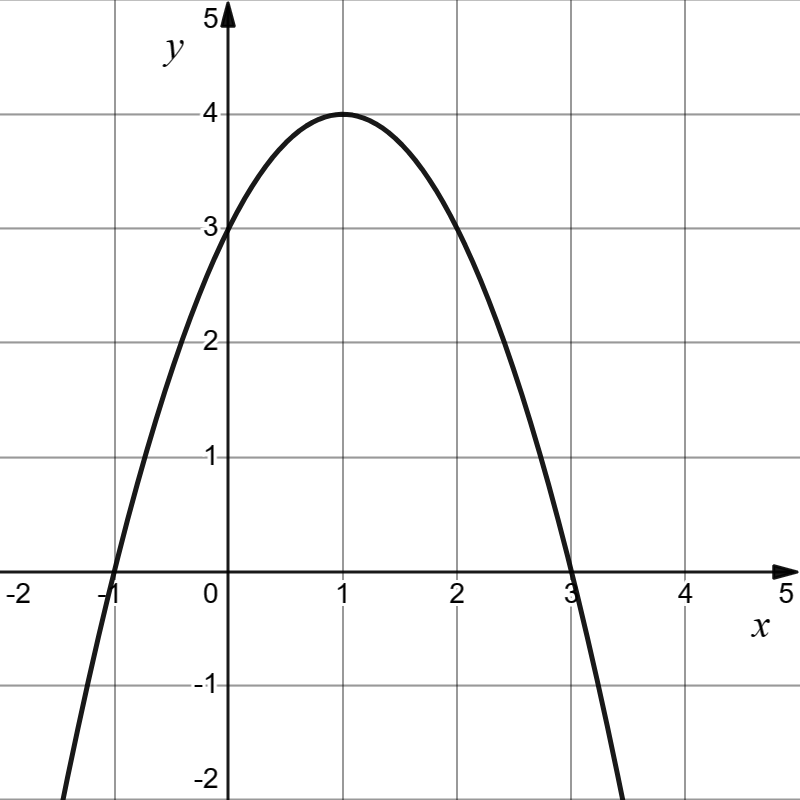
\includegraphics[scale=0.3]{figs/f(x)=-x^2+2x+2.png}
    \end{center}
  \end{multicols}
\end{exercise}
\vspace*{-6\baselineskip}


\newpage

\subsection{Domains and Ranges}




